%!TEX program = xelatex
%Template created by: Maciej Byczko
\documentclass[a4paper,12pt]{extarticle}  %typ dokumentu

% \usepackage[utf8]{inputenc} %rodzaj czcionki w dokumencie
\usepackage{geometry} %poprawienie marginesów
\usepackage{polski} %polskie znaki
\usepackage{multirow} %tabela
\usepackage{graphicx} %tabela
\usepackage{float} %poprawienie pozycji
\usepackage{fancyhdr} % header i footer
\usepackage{karnaugh-map} % rysowanie siatek karnaugh
\usepackage{hyperref} %tworzenie odnośników, \url{<url>}, \href{<file path, link>}{<text with link>} \pageref{}
\usepackage{amsmath} % Matma
\usepackage{boldline}%edytowanie grubości krawędzi w tabelach \hlineB{} \clineB{}{}
\usepackage{array}%grubsze kolumny w tabeli
\usepackage{bigstrut}
\usepackage{caption}
\usepackage{listings} %pisanie kodu w ładny sposób, begin{listings}[language=<język>]...end{listings} tak samo jak nazwa paczki
\usepackage{subcaption}

%Ustawienie paczki hyperref
\hypersetup{
     colorlinks,
     citecolor=black,
     filecolor=black,
     linkcolor=black,
     urlcolor=black
}

\definecolor{backcolour}{rgb}{0.95,0.95,0.92}
\definecolor{AO}{rgb}{0,0.5,0}
\definecolor{ZeroBlue}{rgb}{0,0.28,0.73}
\definecolor{DarkRed}{rgb}{0.85,0.16,0.16}

\lstset{
breaklines=true,
language=vhdl,
numbers=left,
tabsize=2,
numberstyle=\footnotesize,
backgroundcolor=\color{backcolour},
breakatwhitespace=false,
showspaces=false,                
showstringspaces=false,
showtabs=false,
commentstyle=\color{gray},
keywordstyle=\color{ZeroBlue},
% keywordstyle={[2]\color{DarkRed}},
% keywordstyle={[3]\color{ZeroBlue}},
}
\graphicspath{{pictures/}}
\geometry{margin=0.7in}
\pagestyle{fancy}

\cfoot{Strona \thepage}
\rhead{Strona \thepage}
\lhead{\typdoc}
\newcolumntype{?}{!{\vrule width 1.5pt}}

\title{\tytul}
\author{\tworcy}
\date{\data}

%-----------------------PRZYDATNE LINKI----------------------------------
%link do tworzenia tabeli https://tablesgenerator.com
%symbole matematyczne: https://oeis.org/wiki/List_of_LaTeX_mathematical_symbols
%narzędzia matematyczne: https://en.wikibooks.org/wiki/LaTeX/Mathematics
%krótkie podpowiedzi http://www.mif.pg.gda.pl/homepages/sylas/students/wdi/doc/latex-sciaga.html
%symbole do schematów: http://texdoc.net/texmf-dist/doc/latex/circuitikz/circuitikzmanual.pdf
%----------------------------------------------------------------------

%-----------------------SEKCJA DANYCH----------------------------------
\def\tytul{Układy Kombinacyjne i Sekwencyjne w VHDL-u} %<<< tytuł ćwiczenia
\def\nrcw{5} %<<< numer ćwiczenia
\def\data{6 Grudnia 2021r.} %<< data wykonania
\def\prowadzacy{dr inż. Jacek Mazurkiewicz} %<<<prowadzący
\def\nrgrupy{B} %<<<numer grupy
\def\tworcy{Maciej Byczko\\Bartosz Matysiak} %<<< autorzy
\def\zajinfo{PN 10:50 TP} %<<< informacje dotyczące zajęć
\def\typdoc{Sprawozdanie} %<<< typ dokumentu tj Sprawozdanie, zadania itp. {Matematyka dyskretna/Sprawozdanie z Miernictwa}
\begin{document}
\setlength{\headheight}{15pt}

\newcommand{\ov}[1]{\overline{#1} \ }

%-------------------------------------TABELA-DANYCH--------------------------------------------------
\begin{table}[H]
	\centering
	\resizebox{\textwidth}{!}{
		\begin{tabular}{|c|c|c|}\hline
			\begin{tabular}[c]{@{}c@{}}                     \tworcy     \end{tabular} &
			\begin{tabular}[c]{@{}c@{}}Prowadzący:\\        \prowadzacy \end{tabular} &
			\begin{tabular}[c]{@{}c@{}}Numer ćwiczenia\\    \nrcw       \end{tabular}          \\ \hline
			\begin{tabular}[c]{@{}c@{}}                     \zajinfo    \end{tabular} &
			\begin{tabular}[c]{@{}c@{}}Temat ćwiczenia:\\   \tytul      \end{tabular} & Ocena: \\ \hline
			\begin{tabular}[c]{@{}c@{}}Grupa:\\          \nrgrupy    \end{tabular}    &
			\begin{tabular}[c]{@{}c@{}}Data wykonania:\\    \data       \end{tabular} &        \\ \hline
		\end{tabular}}
\end{table}
%----------------------------------------------------------------------------------------------------
\tableofcontents
\cleardoublepage
\section{Zadanie 1}
\subsection{Polecenie}
Implementacja funkcji logicznej \textbf{$G(w,x,y,z) = \prod(0, 2, 3, 4, 6, 7, 9, 11, 12, 13, 15)$} w VHDL-u za pomocą:
\begin{enumerate}
	\item Zapis równań boolowskich
	\item Metoda zapisu tablicowego
\end{enumerate}
\subsection{Rozwiązanie}
\subsubsection{Tabela prawdy}
\begin{table}[H]
	\centering
	\resizebox{0.5\textwidth}{!}{
		\begin{tabular}{?c?c|c|c|c?c?}\hlineB{2.5}
			Kod dziesiętny & w & x & y & z & G \bigstrut \\\hlineB{2.5}
			0              & 0 & 0 & 0 & 0 & 0 \bigstrut \\\hline
			1              & 0 & 0 & 0 & 1 & 1 \bigstrut \\\hline
			2              & 0 & 0 & 1 & 0 & 0 \bigstrut \\\hline
			3              & 0 & 0 & 1 & 1 & 0 \bigstrut \\\hline
			4              & 0 & 1 & 0 & 0 & 0 \bigstrut \\\hline
			5              & 0 & 1 & 0 & 1 & 1 \bigstrut \\\hline
			6              & 0 & 1 & 1 & 0 & 0 \bigstrut \\\hline
			7              & 0 & 1 & 1 & 1 & 0 \bigstrut \\\hline
			8              & 1 & 0 & 0 & 0 & 1 \bigstrut \\\hline
			9              & 1 & 0 & 0 & 1 & 0 \bigstrut \\\hline
			10             & 1 & 0 & 1 & 0 & 1 \bigstrut \\\hline
			11             & 1 & 0 & 1 & 1 & 0 \bigstrut \\\hline
			12             & 1 & 1 & 0 & 0 & 0 \bigstrut \\\hline
			13             & 1 & 1 & 0 & 1 & 0 \bigstrut \\\hline
			14             & 1 & 1 & 1 & 0 & 1 \bigstrut \\\hline
			15             & 1 & 1 & 1 & 1 & 0 \bigstrut \\\hlineB{2.5}
		\end{tabular}%
	}
	\label{zad1-TableTrue}%
\end{table}%
\subsubsection{Siatka Karnaugh}
\begin{figure}[H]
\centering
\resizebox{0.5\textwidth}{!}{
	\begin{karnaugh-map}[4][4][1][$wx$][$yz$]
	\minterms{2,4,5,10,11} % na tych koordynatach umieść jedynki (1)
	\autoterms[0] % umieść ten symbol w miejscach niezdefiniowanych
	\implicant{4}{5} % połącz te komórki
	\implicant{11}{10}
	\implicantedge{2}{2}{10}{10} %połącz komórki brzegowe
	\end{karnaugh-map}
}
\caption{$ Wyj_G = w\overline{x}\overline{z} + \overline{w}\overline{y}z + wy\overline{z}$}
\end{figure}
\subsection{Zapis za pomocą równań boolowskich}
\subsubsection{Kod VHDL}
\lstinputlisting{zadanie1/booleanFunction/gfunction_rownanie_boolowskie.vhd}
\subsection{Kod VHDL TestBench}
\lstinputlisting{zadanie1/booleanFunction/gfunctionTestbench.vhd}
\subsubsection{Symulacja}
\begin{figure}[H]
	\centering
	\resizebox*{\textwidth}{!}{
		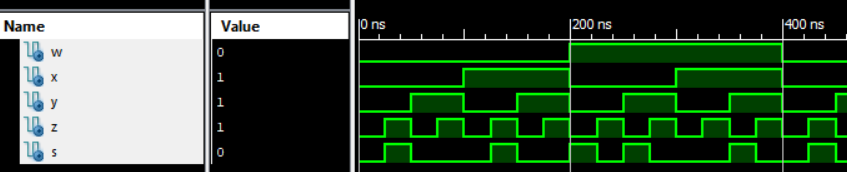
\includegraphics{zadanie1/booleanFunction/przebieg_rownanie_boolowskie.png}
	}
\end{figure}
\subsubsection{Fizyczna implementacja (Kod UCF)}
\lstinputlisting{zadanie1/booleanFunction/ZL-9572.ucf}
\subsection{Zapis tablicowy}
\subsubsection{Kod VHDL}
\lstinputlisting{zadanie1/truthTable/gfunctiontruthtable.vhd}
\subsection{Kod VHDL TestBench}
\lstinputlisting{zadanie1/truthTable/gFunctionTestBenchViaTruthTable.vhd}
\subsubsection{Symulacja}
\begin{figure}[H]
	\centering
	\resizebox*{\textwidth}{!}{
		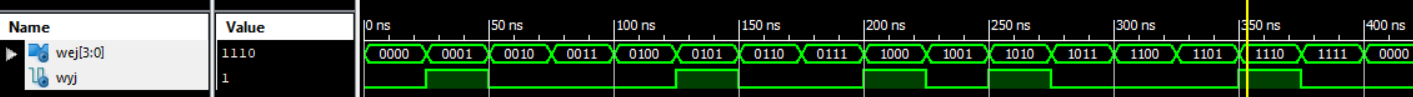
\includegraphics{zadanie1/truthTable/simulation_run.png}
	}
\end{figure}
\subsubsection{Fizyczna implementacja (Kod UCF)}
\lstinputlisting{zadanie1/truthTable/ZL-9572.ucf}
\section{Zadanie 2}
\subsection{Polecenie}
Implementacja układu translatora kodu \textbf{4-bit kod NKB na 4-bit kod Aikena} w VHDL-u za pomocą:
\begin{enumerate}
	\item Zapis równań boolowskich
	\item Metoda zapisu tablicowego
\end{enumerate}
\subsection{Rozwiązanie}
\subsubsection{Tabela prawdy}
\begin{table}[H]
	\centering
	\resizebox{0.5\textwidth}{!}{
		\begin{tabular}{?c?c|c|c|c?c|c|c|c?}\hlineB{2.5}
			\multirow{2}[4]{*}{Kod dziesiętny} & \multicolumn{4}{c?}{NKB} & \multicolumn{4}{c?}{Kod Aikena} \bigstrut                                   \\\clineB{2-9}{2.5}
			                                   & w                        & x                                         & y & z & w & x & y & z \bigstrut \\\hlineB{2.5}
			0                                  & 0                        & 0                                         & 0 & 0 & 0 & 0 & 0 & 0 \bigstrut \\\hline
			1                                  & 0                        & 0                                         & 0 & 1 & 0 & 0 & 0 & 1 \bigstrut \\\hline
			2                                  & 0                        & 0                                         & 1 & 0 & 0 & 0 & 1 & 0 \bigstrut \\\hline
			3                                  & 0                        & 0                                         & 1 & 1 & 0 & 0 & 1 & 1 \bigstrut \\\hline
			4                                  & 0                        & 1                                         & 0 & 0 & 0 & 1 & 0 & 0 \bigstrut \\\hline
			5                                  & 0                        & 1                                         & 0 & 1 & 1 & 0 & 1 & 1 \bigstrut \\\hline
			6                                  & 0                        & 1                                         & 1 & 0 & 1 & 1 & 0 & 0 \bigstrut \\\hline
			7                                  & 0                        & 1                                         & 1 & 1 & 1 & 1 & 0 & 1 \bigstrut \\\hline
			8                                  & 1                        & 0                                         & 0 & 0 & 1 & 1 & 1 & 0 \bigstrut \\\hline
			9                                  & 1                        & 0                                         & 0 & 1 & 1 & 1 & 1 & 1 \bigstrut \\\hline
			10                                 & 1                        & 0                                         & 1 & 0 & - & - & - & - \bigstrut \\\hline
			11                                 & 1                        & 0                                         & 1 & 1 & - & - & - & - \bigstrut \\\hline
			12                                 & 1                        & 1                                         & 0 & 0 & - & - & - & - \bigstrut \\\hline
			13                                 & 1                        & 1                                         & 0 & 1 & - & - & - & - \bigstrut \\\hline
			14                                 & 1                        & 1                                         & 1 & 0 & - & - & - & - \bigstrut \\\hline
			15                                 & 1                        & 1                                         & 1 & 1 & - & - & - & - \bigstrut \\\hlineB{2.5}
		\end{tabular}%
	}
	\label{zad3-TableTrue}%
\end{table}%
\subsubsection{Siatki Karnaugh}
\begin{figure}[H]
\centering
\begin{minipage}[c]{0.4\linewidth}
\begin{karnaugh-map}[4][4][1][$yz$][$wx$]
\maxterms{0,1,2,3,4}
\minterms{5,6,7,8,9}
\implicant{12}{10}
\implicant{5}{15}
\implicant{7}{14}
\autoterms[-]
\end{karnaugh-map}
\caption*{$w_A = xz + xy + w$}
\end{minipage}
\begin{minipage}[c]{0.4\linewidth}
\begin{karnaugh-map}[4][4][1][$yz$][$wx$]
\maxterms{0,1,2,3,5}
\minterms{4,6,7,8,9}
\implicant{12}{10}
\implicant{7}{14}
\implicantedge{4}{12}{6}{14}
\autoterms[-]
\end{karnaugh-map}
\caption*{$x_A = x\overline{z} + xy + w$}
\end{minipage}
\end{figure}

\begin{figure}[H]
\centering
\begin{minipage}[c]{0.4\linewidth}
\begin{karnaugh-map}[4][4][1][$yz$][$wx$]
\maxterms{0,1,4,6,7}
\minterms{2,3,5,8,9}
\implicant{12}{10}
\implicant{5}{13}
\implicantedge{3}{2}{11}{10}
\autoterms[-]
\end{karnaugh-map}
\caption*{$y_A = \overline{x}y + x\overline{y}z + w$}
\end{minipage}
\begin{minipage}[c]{0.4\linewidth}
\begin{karnaugh-map}[4][4][1][$yz$][$wx$]
\maxterms{0,2,4,6,8}
\minterms{1,3,5,7,9}
\implicant{1}{11}
\autoterms[-]
\end{karnaugh-map}
\caption*{$z_A = z$}
\end{minipage}

\end{figure}
\subsection{Zapis za pomocą równań boolowskich}
\subsubsection{Kod VHDL}
\lstinputlisting{zadanie2/boolean/boolean_aiken.vhd}
\subsection{Kod VHDL TestBench}
\lstinputlisting{zadanie2/boolean/boolean_aiken_testbench.vhd}
\subsubsection{Symulacja}
\begin{figure}[H]
	\centering
	\resizebox*{\textwidth}{!}{
		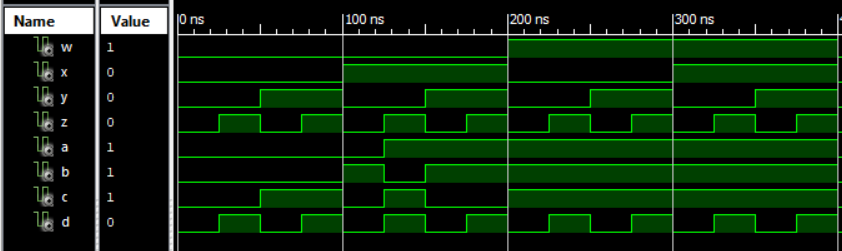
\includegraphics{zadanie2/boolean/simulation_boolean_equation.png}
	}
\end{figure}
\subsubsection{Fizyczna implementacja (Kod UCF)}
\lstinputlisting{zadanie2/boolean/ZL-9572.ucf}
\subsection{Zapis tablicowy}
\subsubsection{Kod VHDL}
\lstinputlisting{zadanie2/table/table_aiken.vhd}
\subsection{Kod VHDL TestBench}
\lstinputlisting{zadanie2/table/table_aiken_testbench.vhd}
\subsubsection{Symulacja}
\begin{figure}[H]
	\centering
	\resizebox*{\textwidth}{!}{
		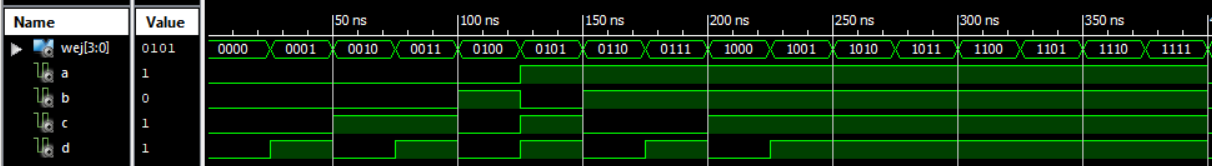
\includegraphics{zadanie2/table/simulation_table_method.png}
	}
\end{figure}
\subsubsection{Fizyczna implementacja (Kod UCF)}
\lstinputlisting{zadanie2/table/ZL-9572.ucf}

\section{Zadanie 3}
\subsection{Polecenie}
Detektor sekwencji 11011, automat Mealy-ego, jedno wejście, jedno wyjście, brak resetu, sekwencja prawidłowa 5-bitowa w VHDL-u jako maszyna stanów.
\subsection{Rozwiązanie}
\subsubsection{Opis symboliki}
\textbf{Alfabet wejściowy}
\begin{itemize}
	\item $z_0 = 0$
	\item $z_1 = 1$
\end{itemize}
\textbf{Stany wewnętrzne}
\begin{itemize}
	\item $q_0$ - stan początkowy | wprowadzono niepoprawny ciąg bitów
	\item $q_1$ - wprowadzono pierwszą cyfrę prawidłowego ciągu
	\item $q_2$ - wprowadzono drugą cyfrę prawidłowego ciągu
	\item $q_3$ - wprowadzono trzecią cyfrę prawidłowego ciągu
	\item $q_4$ - wprowadzono czwartą cyfrę prawidłowego ciągu
	\item $q_5$ - wprowadzono poprawną sekwencję
\end{itemize}
\textbf{Alfabet wyjścia}
\begin{itemize}
	\item $y_0$ - Wprowadzony ciąg nadal jest niepoprawny
	\item $y_1$ - Wprowadzono poprawną sekwencję
\end{itemize}
\subsubsection{Schemat grafowy}
\begin{figure}[H]
	\centering
	\resizebox*{\textwidth}{!}{
		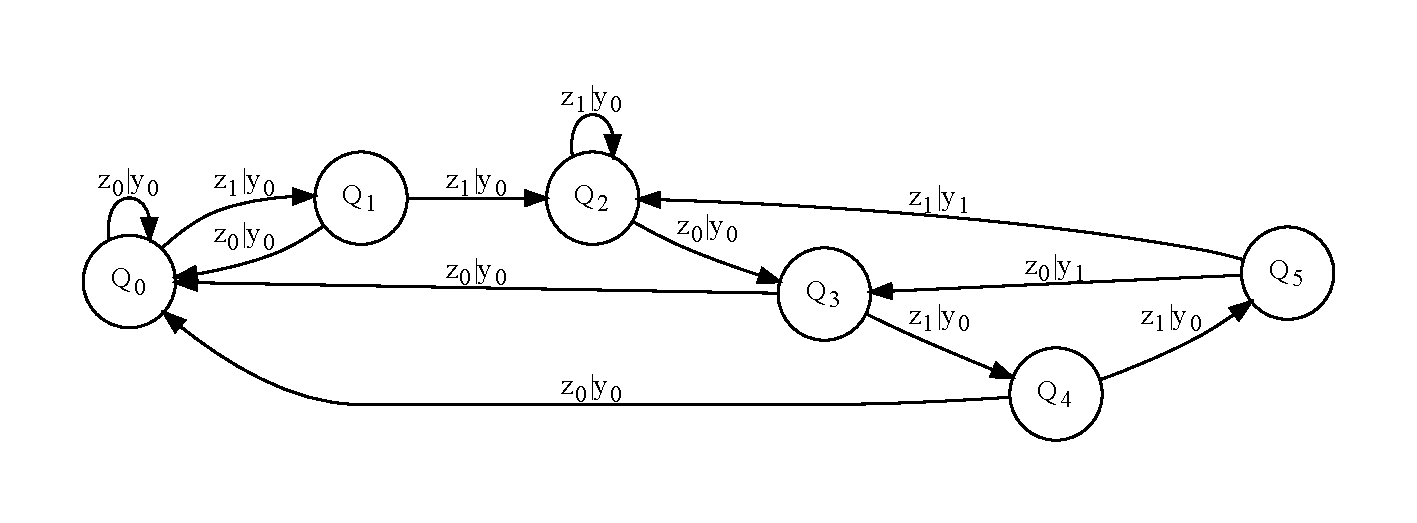
\includegraphics{zadanie3/mealy.pdf}
	}
\end{figure}
\subsubsection{Tabela prawdy}
\begin{table}[H]
	\centering
	\resizebox*{0.8\textwidth}{!}{
		\begin{tabular}{|c?c|c|c?c?c|c|c?c?c|c|c|}
			\hline
			\multirow{2}[4]{*}{S}                                 & \multicolumn{3}{c?}{Q(t)} & \multirow{2}[4]{*}{Z} & \multicolumn{3}{c?}{Q(t+1)} & \multirow{2}[4]{*}{Y}                                      \\
			\clineB{2-4}{2.5}\clineB{6-8}{2.5}\clineB{10-12}{2.5} & $Q_2$                     & $Q_1$                 & $Q_0$                       &                       & $Q_2$ & $Q_1$ & $Q_0$ & \bigstrut   \\
			\hlineB{2.5}
			$Q_0$                                                 & 0                         & 0                     & 0                           & 0                     & 0     & 0     & 0     & 0          \\\hline
			$Q_0$                                                 & 0                         & 0                     & 0                           & 1                     & 0     & 0     & 1     & 0          \\\hline
			$Q_1$                                                 & 0                         & 0                     & 1                           & 0                     & 0     & 0     & 0     & 0          \\\hline
			$Q_1$                                                 & 0                         & 0                     & 1                           & 1                     & 0     & 1     & 0     & 0          \\\hline
			$Q_2$                                                 & 0                         & 1                     & 0                           & 0                     & 0     & 1     & 1     & 0          \\\hline
			$Q_2$                                                 & 0                         & 1                     & 0                           & 1                     & 0     & 1     & 0     & 0          \\\hline
			$Q_3$                                                 & 0                         & 1                     & 1                           & 0                     & 0     & 0     & 0     & 0          \\\hline
			$Q_3$                                                 & 0                         & 1                     & 1                           & 1                     & 1     & 0     & 0     & 0          \\\hline
			$Q_4$                                                 & 1                         & 0                     & 0                           & 0                     & 0     & 0     & 0     & 0          \\\hline
			$Q_4$                                                 & 1                         & 0                     & 0                           & 1                     & 1     & 0     & 1     & 0          \\\hline
			$Q_5$                                                 & 1                         & 0                     & 1                           & 0                     & 0     & 1     & 1     & 1          \\\hline
			$Q_5$                                                 & 1                         & 0                     & 1                           & 1                     & 0     & 1     & 0     & 1          \\\hline
			-                                                     & 1                         & 1                     & 0                           & 0                     & -     & -     & -     & -          \\\hline
			-                                                     & 1                         & 1                     & 0                           & 1                     & -     & -     & -     & -          \\\hline
			-                                                     & 1                         & 1                     & 1                           & 0                     & -     & -     & -     & -          \\\hline
			-                                                     & 1                         & 1                     & 1                           & 1                     & -     & -     & -     & -          \\\hline
		\end{tabular}%
	}
	\label{tab:mealy}%
\end{table}%

\subsubsection{Kod VHDL}
\lstinputlisting{zadanie3/detectormodule.vhd}
\subsubsection{Kod VHDL TestBench}
\lstinputlisting{zadanie3/detectorTestBench.vhd}
\subsubsection{Symulacja}
\begin{figure}[H]
   \centering
   \resizebox*{\textwidth}{!}{
	  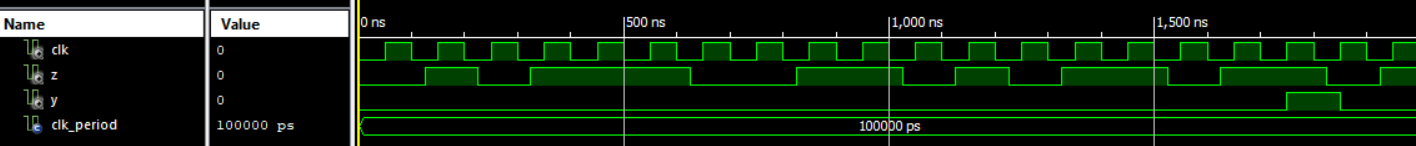
\includegraphics{zadanie3/simulation_run.png}
   }
\end{figure}
\subsubsection{Fizyczna implementacja (Kod UCF)}
\lstinputlisting{zadanie3/ZL-9572.ucf}
\section{Zadanie 4}
\subsection{Polecenie}
Zaprojektować licznik synchroniczny liczący w tył na bazie kodu Aikena w zakresie 0-6 (mod 7) jako maszyna stanów.
\subsection{Rozwiązanie}
\subsubsection{Schemat stanów}
\begin{figure}[H]
	\centering
	\resizebox*{0.65\textwidth}{!}{
		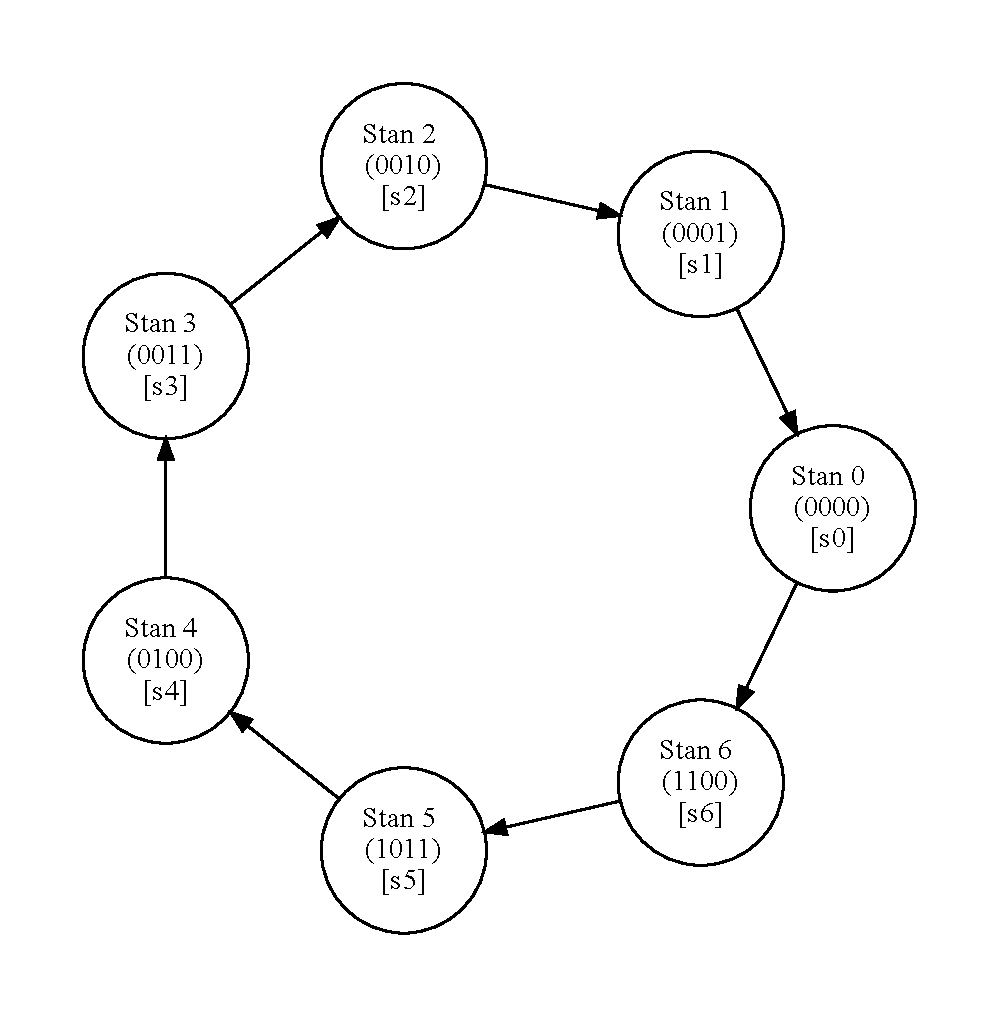
\includegraphics{zadanie4/stany2.pdf}
	}
\end{figure}
\subsubsection{Tabela prawdy}
\begin{table}[H]
	\centering
	\resizebox{\textwidth}{!}{
		\begin{tabular}{|c?c|c|c|c?c|c|c|c|}
			\hline
			\multirow{2}[3]{*}{n} & \multicolumn{4}{c?}{Q(t)} & \multicolumn{4}{c?}{Q(t+1)}                                                \\
			\clineB{2-9}{2.5}    & $Q_3$                     & $Q_2$                       & $Q_1$ & $Q_0$ & $Q_3$ & $Q_2$ & $Q_1$ & $Q_0$ \\\hlineB{2.5}
			0                     & 0                         & 0                           & 0     & 0     & 1     & 1     & 0     & 0     \\\hline
			1                     & 0                         & 0                           & 0     & 1     & 0     & 0     & 0     & 0     \\\hline
			2                     & 0                         & 0                           & 1     & 0     & 0     & 0     & 0     & 1     \\\hline
			3                     & 0                         & 0                           & 1     & 1     & 0     & 0     & 1     & 0     \\\hline
			4                     & 0                         & 1                           & 0     & 0     & 0     & 0     & 1     & 1     \\\hline
			5                     & 1                         & 0                           & 1     & 1     & 0     & 1     & 0     & 0     \\\hline
			6                     & 1                         & 1                           & 0     & 0     & 1     & 0     & 1     & 1     \\\hline
		\end{tabular}%
	}
	\label{tab:states}%
\end{table}%
\subsubsection{Kod VHDL}
\lstinputlisting{zadanie4/aiken_counter.vhd}
\subsubsection{Kod VHDL Testbench}
\lstinputlisting{zadanie4/aiken_counter_testbench.vhd}
\subsubsection{Symulacja}
\begin{figure}[H]
   \centering
   \resizebox*{\textwidth}{!}{
	  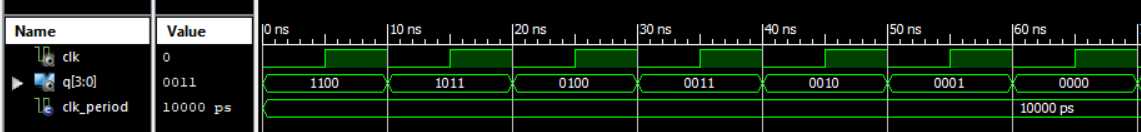
\includegraphics{zadanie4/simulation_aiken_counter.png}
   }
\end{figure}
\subsubsection{Fizyczna implementacja (Kod UCF)}
\lstinputlisting{zadanie4/ZL-9572.ucf}

\section{Wnioski}

Na początku trudność sprawiło nam testowanie modułów w języku VHDL. Problem rozwiązał się sam, w momencie, gdy natknięcia się na materiał instruktażowy, w którym pokazane zostało, że przy testowaniu modułu, plik testowy vhd należy wygenerować na podstawie napisanego modułu (sam moduł nie stanowi pliku testowego).

\end{document}